

\documentclass[12pt,a4paper]{book}



			% Packages Files
%----------------------------------%

	% Page Setttings
\usepackage[top = 1in, bottom = 1in, left = 1in, right = 1in]{geometry}

\parindent=0cm % to prevent the spacing in new paragraph or new line

\usepackage{fancyhdr} % needded for header and footer 

%-----------------------------------------------------------------%

\usepackage{amsmath} % needed for referencing thequation
\usepackage{amsfonts} % for maths symbols
\usepackage{graphicx}
\usepackage[export]{adjustbox}
\usepackage{caption}
\usepackage{refstyle} % to reference a captioned figure


% To make hyperlinks

\usepackage[
	colorlinks=true
	,breaklinks
	]{hyperref} % needed for creating hyperlinks in the document, the option colorlinks=true gets rid of the awful boxes, breaklinks breaks lonkg links (list of figures),
	
\usepackage{xcolor}
\definecolor{c1}{rgb}{0,0,1} % blue
\definecolor{c2}{rgb}{0,0.3,0.9} % light blue
\definecolor{c3}{rgb}{0.3,0,0.9} % red blue
\hypersetup{
    linkcolor={c1}, % internal links
    citecolor={c2}, % citations
    urlcolor={c3} % external links/urls
}

	% For Code Writing
	
\usepackage{listings}

\usepackage{color}

\definecolor{mygreen}{rgb}{0 0.6 0}

\lstset{
% Set automatic Line breaking, in case we have long lines don't
% fit inside the frame or the page.
breaklines = true,
commentstyle = \color{mygreen},
breakatwhitespace = true,% don't show white space character
%numbers = left, % put line number in the code
title = \lstname
}

% ------------- For Writing Equations inisde a table and centering them ------------

\usepackage{array}

% Vertical Alignment inside the cells of the table
\newcolumntype{M}[1]{>{\centering\arraybackslash}m{#1}}

% Horizontal Alignment inside the cells of the table
\newcolumntype{P}[1]{>{\centering\arraybackslash}p{#1}}


% needed for todos liste
\usepackage{todonotes} 


\usepackage{nomencl}



% Macros File

% Macros Example
\def\labelaxes{Remember to include some suitable labeling for the axes and the units used in measurements.}

% 2nd way for defnining macros: the new command
% 1st parameter: name of the new command
% 2nd paramter: how many inputs this command needs, in this case only 1
% 3rd parameter: what this new command named \tbi do

\newcommand{\tbi}[1]{\textbf{\textit{#1}}}

% Command for Picture without a label

\newcommand{\pic}[3]{\begin{figure}[h]
\centering
\includegraphics[width = 0.7\textwidth, frame]{#1}
\caption{#2}
\end{figure}}








\DeclareMathOperator*{\argmax}{argmax} % thin space, limits underneath in displays

\DeclareMathOperator*{\argmin}{argmin}

\title{Signal Processing Summary}
\author{Ranim Tom}



\begin{document}

% downloaded template
%\input{content/title_page_1} 

\maketitle
\tableofcontents




\pagestyle{fancy}
\fancyhf{} % Clear header and footer
\rhead{\rightmark}
\lhead{Chapter \thechapter}
\rfoot{Page \thepage}


\chapter{Abstract}

This document contains summary and key ideas for \tbi{signal processing}.\\

It is not meant to be an detailed reference (where proofs and detailed explanation are presented). For this purpose, references to my course reader and references.

\chapter{Sampling and Reconstruction}


\section{Impulse Sampling of Continuous Time Signal}

Let $x(t) \, \leftrightarrow \, X(\omega)$ be a continuous time signal with its associated Fourier transform $X(\omega)$.\\

\underline{Effect of doing impulse sampling to $x(t)$:}\\

Let $x_{\delta}(t)$ the sampled impulse signal where:

\begin{equation}
\begin{array}{rcl}
x_{\delta}(t) \, &=& \, x(t) \, \times \, p(t) \\ \\
				&=& \, x(t) \, \times \, \displaystyle\sum\limits_{n \, = \, - \infty}^{+ \infty} \delta (t \, - \, n \, T_s)
\end{array}
\end{equation}
 
$p(t)$ is \tbi{train of pulses} located at multiple of $T_s$.\\



\begin{figure}[h]
\centering
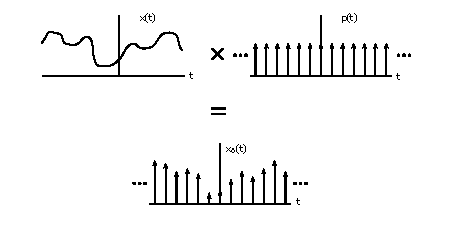
\includegraphics[width = 0.7\textwidth, frame]{Figures/Sampling/impulse_sampling}
\caption{Impulse Sampling of a continuous time signal}
\label{fig:Sampling:impulse_sampling}
\end{figure}


\newpage
In the frequency domain, this will change $X(\omega)$ to be $X_{\delta}(\omega)$ as shown in \autoref{fig:Sampling:impulse_sampling_spectrum_1}.


\begin{figure}[h]
\centering
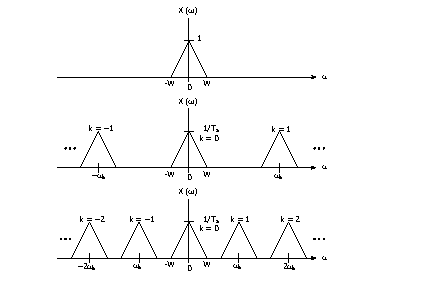
\includegraphics[width = 0.7\textwidth, frame]{Figures/Sampling/impulse_sampling_spectrum_1}
\caption{Sampling Higher then the Nyquite Rate}
\label{fig:Sampling:impulse_sampling_spectrum_1}
\end{figure}



\begin{itemize}

\item  Equation:

\begin{equation}
\begin{array}{rcl}
X_{\delta}(\omega_c) \, &=& \, \displaystyle\frac{1}{2 \, \pi} X(\omega_c) \, * \, P(\omega_c) \\ \\
				&=& \,\displaystyle\frac{1}{T_s} \displaystyle\sum\limits_{k \, = \, - \infty}^{+ \infty} X (\omega \, - \, k \, \omega_s)
\end{array}
\end{equation}


\item So when we do impulse sampling, the spectrum of $X(\omega_c)$ will be replicated with multiple of $\omega_s$.


\item Notice that also $X_{\delta}(\omega)$ has a \tbi{scaling factor} equal to $\displaystyle\frac{1}{T_s}$.

	\begin{itemize}
	\item This scaling factor is \tbi{an amplitude distortion factor} since the original spectrum $X(\omega)$ didn't has such a factor.
	\end{itemize}

\end{itemize}

\newpage
\subsection{Aliasing Effect}


\underline{Definition:} The replications (at multiple of $\omega_s$) of the spectrum overlap with the original spectrum,as shown in \autoref{fig:Sampling:impulse_sampling_spectrum_2}.

\begin{figure}[h]
\centering
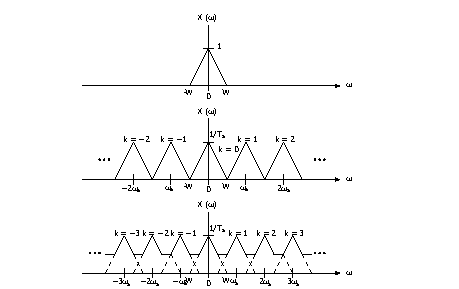
\includegraphics[width = 0.7\textwidth, frame]{Figures/Sampling/impulse_sampling_spectrum_2}
\caption{Decreasing the Nyquist Rate: Aliasing Result}
\label{fig:Sampling:impulse_sampling_spectrum_2}
\end{figure}

\begin{itemize}

\item When decreasing the sampling rate $\omega_s$, the shifted spectrum get close to each other

	\begin{itemize}
	\item In the $\mathrm{2}^\mathrm{nd}$ row of \autoref{fig:Sampling:impulse_sampling_spectrum_2}, we are \tbi{sampling exactly at the Nyquist rate}
	
	\item \tbi{No gap} between the original spectrum and the shifted version
	\end{itemize}


\item When sampling rate $\omega_s$ \tbi{less then the Nyquist rate}, the \tbi{shifted versions} have \tbi{collide} with the original spectrum 

	\begin{itemize}
	\item The only thing we can see is the blue solid line
	
	\item We could not retrieve the original spectrum as before now.
	\end{itemize}

\end{itemize}

\underline{Note:} 

\begin{itemize}

\item Review the cosine sampling example at all cases of $\omega_s$, very important example illustrating the effect of sampling.

\item Also the example about predicting the aliasing frequency


\begin{equation}
\begin{array}{rcl}
f_{\text{alias}} \, &\leq& \, \displaystyle\frac{Fs}{2} \\
f_{\text{alias}} \, &=& \, \lvert f_{\text{original}} \, - \, m \, f_s  \rvert \quad \text{where } m \, = \, 0 \, ; \, 1 \, ; \, 2 ;\, \cdots
\end{array}
\label{Eq:Sampling:alias_frequency}
\end{equation}

\end{itemize}



\newpage
\section{Practical Sampling: ZOH}

\begin{itemize}

\item Another method to get samples from a continuous signal, shown in \autoref{fig:Sampling:sampling_zoh}.

\begin{figure}[h]
\centering
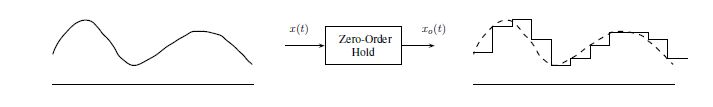
\includegraphics[width = 0.7\textwidth, frame]{Figures/Sampling/sampling_zoh}
\caption{Sampling using ZOH}
\label{fig:Sampling:sampling_zoh}
\end{figure}

\item Why called ZOH:

	\begin{itemize}
	\item this filter grab a value of the signal, and then hold this value till it grab the next value
	
	\item  returns a \tbi{stair case like signal}, where each value of the signal is held till the next sampling time occurred
	\end{itemize}


\item In other words, instead of having ideal sampling denoted as $x[k]$, we will have a convolution with a shifted square pulse $x(t) \, \star \, h_{\text{ZOH}}(t)$ where $h_{\text{ZOH}}(t)$ is the impulse response of the ZOH sampler

    \begin{itemize}
        \item The shifting is because the sampler is causal
        
        \item More complicated kernel for more complex type of interpolation, like triangular pulse for linear interpolation
    \end{itemize}

\item Mathematical modeling of the ZOH is shown in \autoref{fig:Sampling:zoh_math}. 


\begin{figure}[h]
\centering
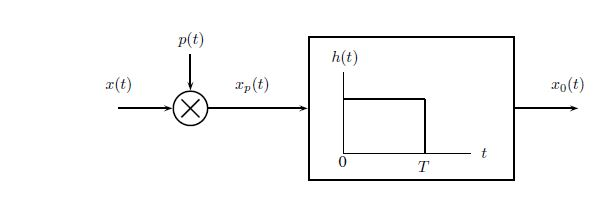
\includegraphics[width = 0.7\textwidth, frame]{Figures/Sampling/zoh_math}
\caption{Mathematical modeling of the ZOH}
\label{fig:Sampling:zoh_math}
\end{figure}

See the book for the detailed description.


\item Spectrum of the Signal Compared to Impulse sampling of \autoref{fig:Sampling:impulse_sampling_spectrum_1}

Spectrum of the signal $x(t)$ using ZOH is shown in \autoref{fig:Sampling:zoh_output_spectrum}.

\begin{figure}[h]
\centering
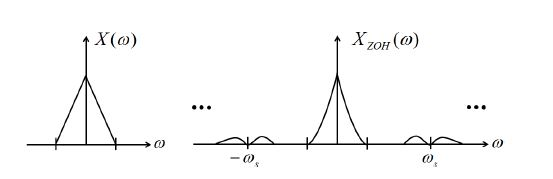
\includegraphics[width = 0.7\textwidth, frame]{Figures/Sampling/zoh_output_spectrum}
\caption{Output of ZOH in the frequency domain}
\label{fig:Sampling:zoh_output_spectrum}
\end{figure}

\begin{itemize}

\item In impulse sampling (see \autoref{fig:Sampling:impulse_sampling_spectrum_1}), the spectrum was the same (with the scale factor $\displaystyle\frac{1}{T_s}$), along with the replicate at multiple of $\omega_s$.


\item In ZOH, these replicate are attenuated due to the low pass nature of the ZOH, which is a good thing since we don't want these images.

\item However, the original spectrum is getting distorted, and this distortion is controlled by the time sampling we choose to get our values. 

\end{itemize}

\end{itemize}


\underline{Sampling Cos Signal Demo:}\\

\begin{figure}[h]
\centering
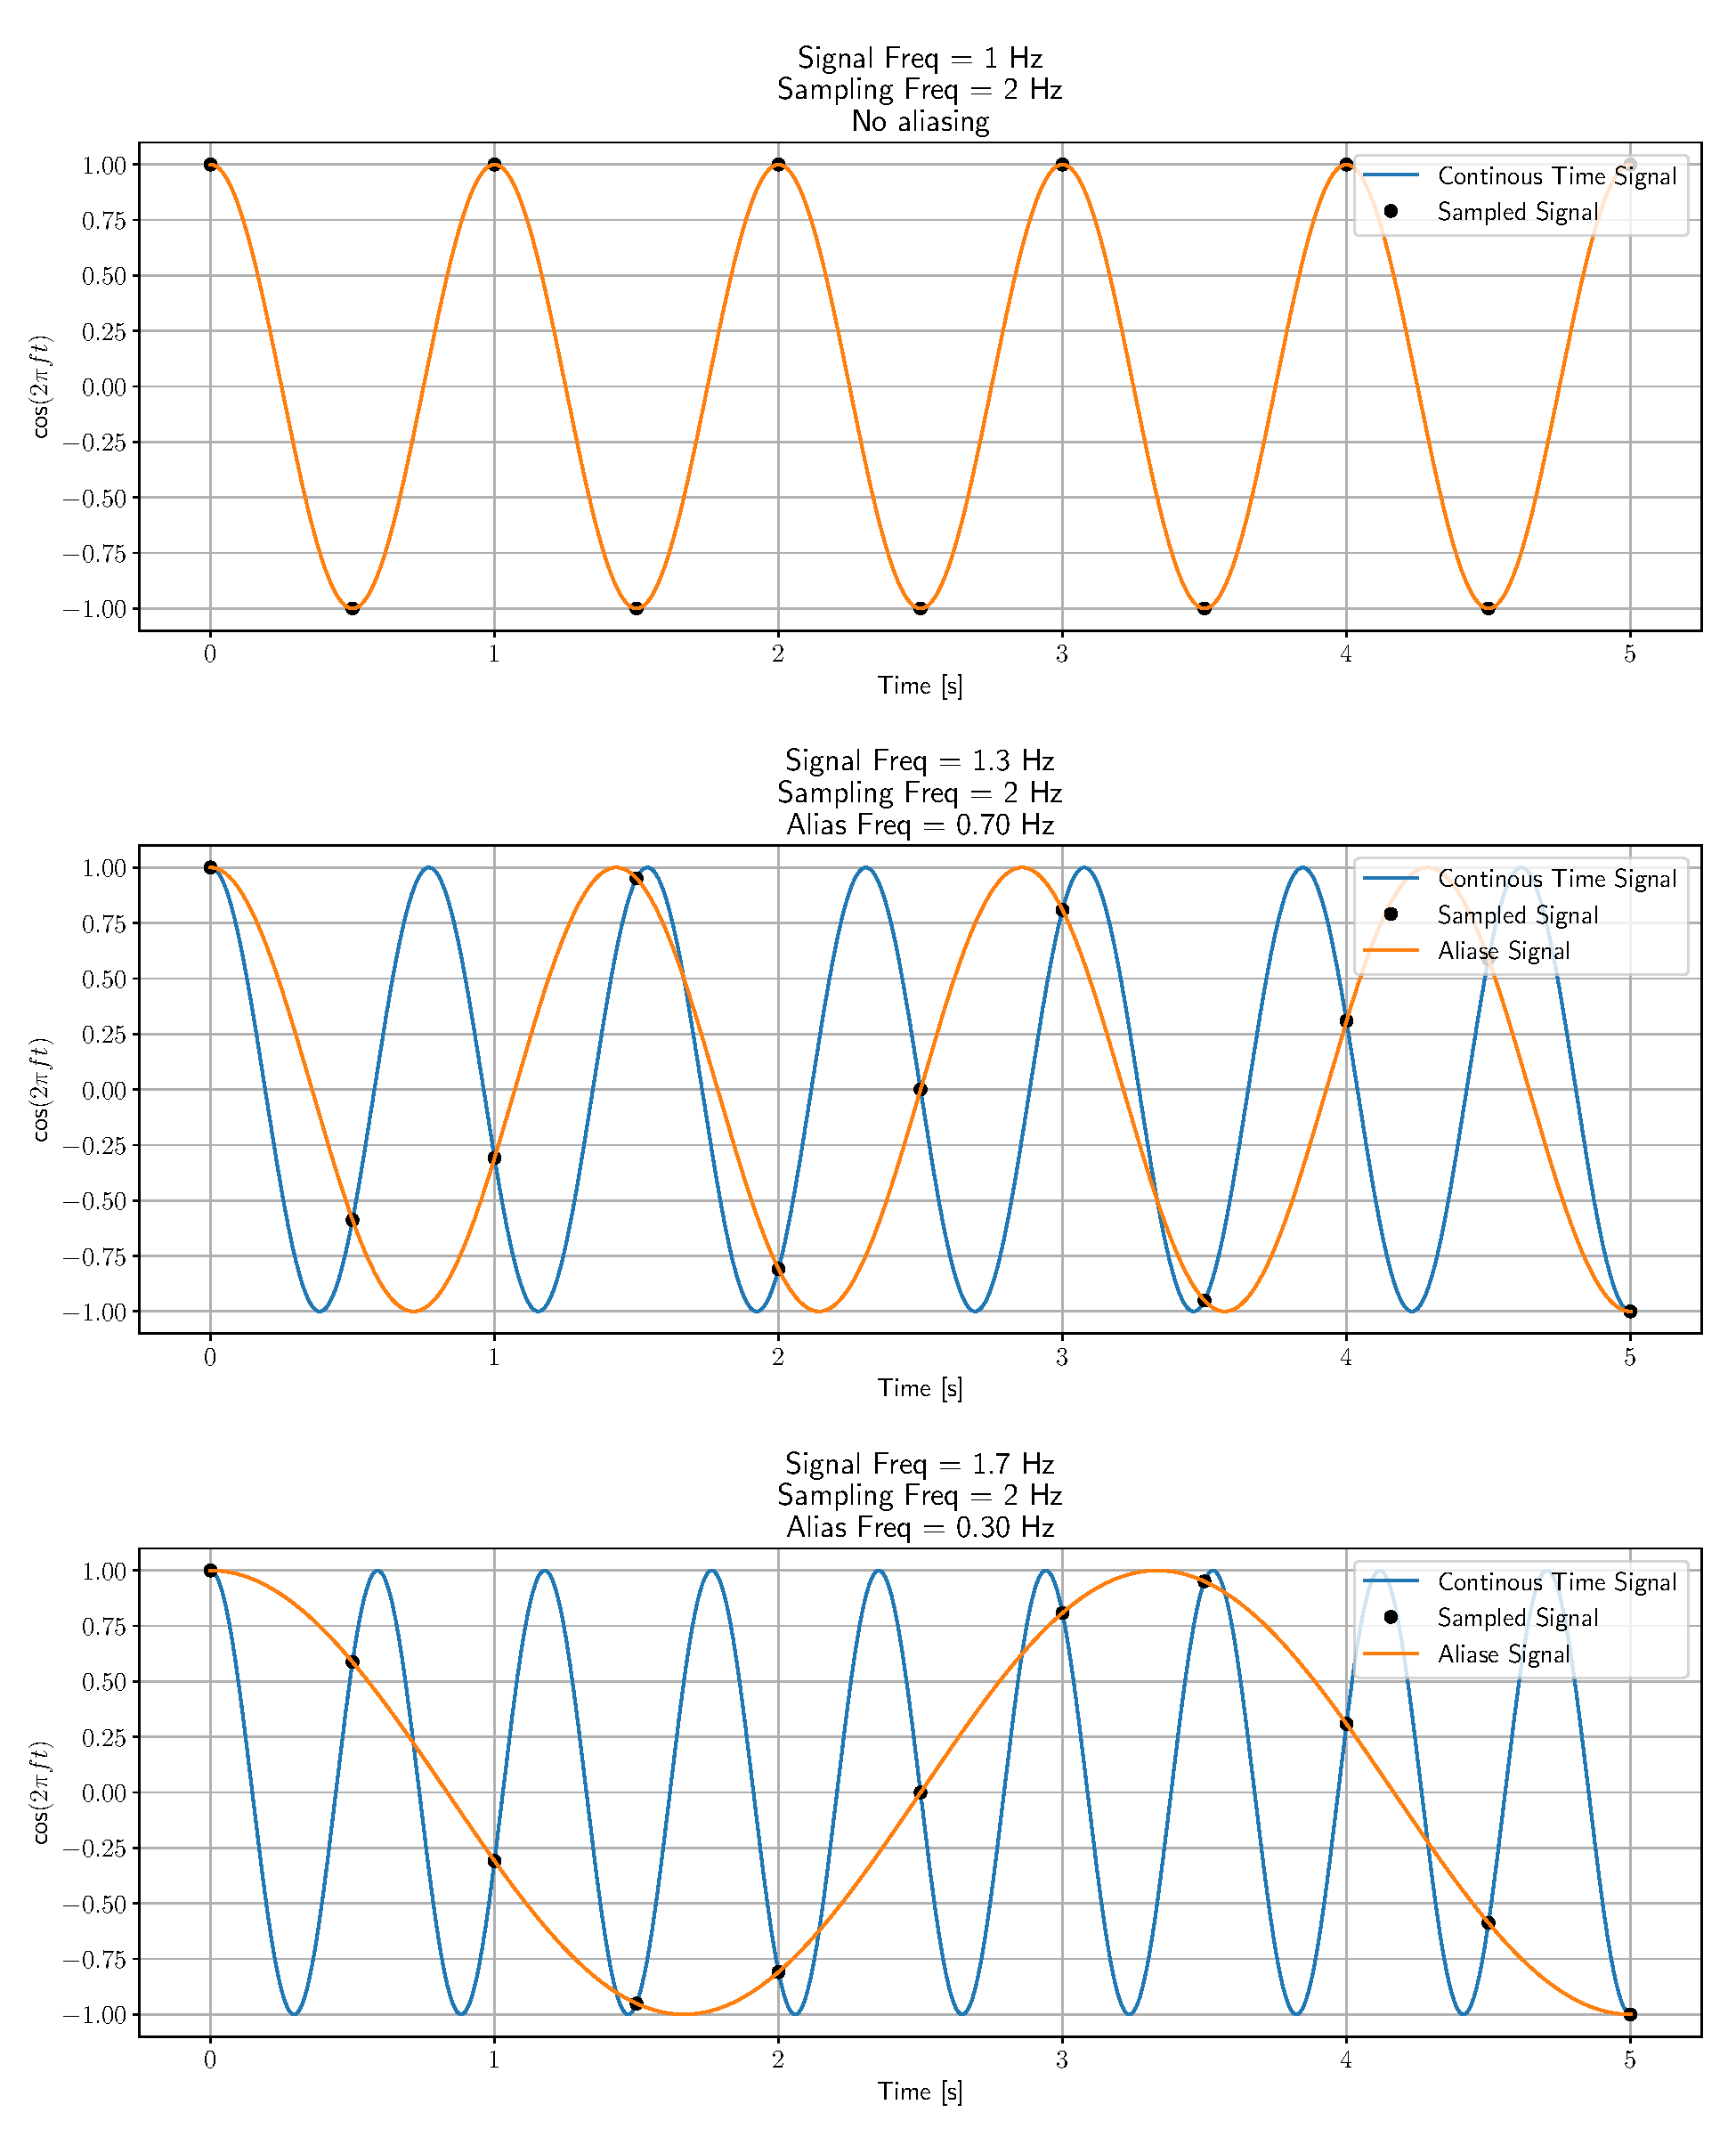
\includegraphics[width = 0.7\textwidth, frame]{Figures/Sampling/Signal_Cont_and_sampled}
\caption{Demonstration of aliasing effect}
\label{fig:Sampling:Signal_Cont_and_sampled}
\end{figure}

\begin{itemize}

\item $F_s \, = \, 2$ Hz

\item We fixed $F_s$ and change the frequency of the cos signal

	\begin{itemize}
	\item The more the $f_{\text{signal}}$ increased and get close to the $F_s$, the $f_{\text{alias}}$ decrease, hence a slower cos version appear 
	\end{itemize}


\end{itemize}

\section{DT Processing for CT Systems}

\begin{itemize}
    
\item Processing continuous time signals using discrete time system (filters) is more beneficial (uses of DSP,$\cdots$)

\item The steps is shown in \autoref{fig:Sampling:discrete_time_processing_for_continious_time}

\begin{figure}[h]
\centering
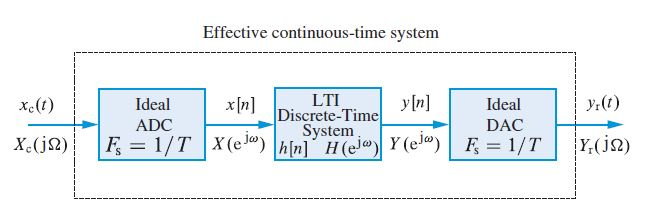
\includegraphics[width = 0.7\textwidth, frame]{Figures/Sampling/discrete_time_processing_for_continious_time}
\caption{Demonstration of aliasing effect}
\label{fig:Sampling:discrete_time_processing_for_continious_time}
\end{figure}

    \begin{itemize}
        \item The input and output are some analog signals
        
        \item The system $H(\omega_d)$ is a discrete time filter (system)
    
    \end{itemize}

\item Several steps to arrive from $x_c(t) \, \rightarrow \, y_c(t)$

    \begin{enumerate}
    
    \item ADC operation: which involve multiplying $x_c(t)$ by a stream of $\delta(t)$ with a period of $T_s$
    
    \item Obtaining the discrete time signal $x[n]$
    
    \item Processing through $h[n]$
    
    \item DAC: reconstruct through a sinc interpolator $\leftrightarrow$ a low pass filter of cuttoff frequency $\displaystyle\frac{\pi}{T_s} \, \equiv \, \displaystyle\frac{F_s}{2}$
    
    \end{enumerate}
    
\item We can simplify all these steps by constructing some equivalent continuous time system $H_{\text{equiv}}(\omega_c)$, which is defined as (proof in \cite{DSP_DimitrisManolakis}, section 6.4)    

\begin{equation}
 H_{\text{equiv}}(\omega_c) \, = \, \begin{cases}
 H(\omega_d) \quad \text{for } \rvert \omega_c \lvert \, \leq \, \displaystyle\frac{\pi}{T_s} \\
 0 \quad \text{for }  \rvert \omega_c \lvert \, > \, \displaystyle\frac{\pi}{T_s}
 \end{cases}
\end{equation}

For a low pass filter, we have:

\begin{equation}
 H_{\text{equiv}}(\omega_c) \, = \, \begin{cases}
1 \quad \text{for } \rvert \omega_c \lvert \, \leq \, \displaystyle\frac{\omega_c}{T_s} \\
 0 \quad \text{for }  \rvert \omega_c \lvert \, > \, \displaystyle\frac{\omega_c}{T_s}
 \end{cases}
\end{equation}

\item Big Conclusion and Key idea: we can use the same discrete time low pass filter of cuttoff frequency $\omega_c$, to implement various analog LPF by changing only the sampling period $T_s$

\end{itemize}


%********************************************
%********************************************
%********************************************

\chapter{DFT and FFT Processing}


\section{Recap of Fourier Transform}

\todo{Fourier Transform Formula}: to put all formula here.

\section{DFT Formula}

Let $f[k]$ a discrete signal with index $k$, of length $N_0$.

\begin{equation}
\begin{array}{rcl}
\text{DFT}\{f[k]\} \, &=&\, F_r \\
						&=& \, F(r \, \Omega_0) \\
					   &=&\, \displaystyle\sum_{k \, = \, 0}^{N_0 \, - \, 1} \, f[k] \, \text{exp} \left(\, -j r \Omega_0 \, k   \,\right)
\end{array}
\label{Eq:DFT:dft_for_dtft}
\end{equation}
 
where $\begin{cases}
r \, = \, 0,1,2, \rightarrow \, N_0 \, - \, 1 \\
\Omega_0 \, = \,  \displaystyle\frac{2 \, \pi}{N_0} \, = \, \text{freqeuncy step at which we sample the DTFT spectrum}
\end{cases}$\\


\underline{Inverse DFT case:}\\

\begin{equation}
\begin{array}{rcl}
f[k] \, &=&\, \displaystyle\frac{1}{N_0} \, \displaystyle\sum_{r \, = \, 0}^{N_0 \, - \, 1} \, F_r \, \text{exp} \left(\, -j r \Omega_0 \, k   \,\right)
\end{array}
\end{equation}


\section{Frequency Variables}

\begin{itemize}

\item Relation between \textit{normalized angular frequency} $\omega$ [rad/cycle] and \textit{continuous angular frequency} $\Omega$ [rad/s] \cite{DSP_DimitrisManolakis}
    
\begin{equation}
    \omega  = \displaystyle\frac{\Omega}{F_s} 
\end{equation}

\item Moving between Hz and radian/cycle

\begin{itemize}
    \item From Hz $\rightarrow$ radian/cycle
    
    \begin{equation}
        \omega \, [\text{radian/cycle}] \, = \, F [\text{Hz}] \, \times \, \left( \, \displaystyle\frac{2 \pi}{F_s} \, \right)
    \end{equation}
    
    \item From radian/cycle $\rightarrow$  Hz
    
    \begin{equation}
        F \, [\text{Hz}] \, = \, \omega [\text{radian/cycle}] \, \times \, \left( \, \displaystyle\frac{F_s}{2 \pi} \, \, \right)
    \end{equation}
    
    
\end{itemize}


\end{itemize}

\section{DTFT-CTFT Relation}

See \cite{signal_processing_Lathi}.

\begin{equation}
\begin{array}{lll}
X_{\delta}(F) \, &=& \, \displaystyle\frac{1}{T_s} \displaystyle\sum\limits_{k \, = \, -\infty}^{+ \infty} X_c \left(\, F \, - \, k \,F_s  \,\right) \\ \\
                &=& \, X(\omega)
\end{array}
\label{Eq:DTFT-CTFT-Relation}
\end{equation}

\begin{itemize}
    \item $X(\omega)$ is an DTFT of $x[n] \leftrightarrow$ DTFT of a discrete signal
    
    \item $X_c(F)$: CTFT of the $x(t) \leftrightarrow$ CTFT of a analog continous signal
    
    \item $X_{\delta}(F)$: CTFT of $x(n \, T_s) \leftrightarrow$ CTFT of a sampled signal 
    
\end{itemize}

\autoref{Eq:DTFT-CTFT-Relation} states that DTFT and CTFT of a sampled signal are the same, and if we want to retrieve the CTFT of $x(t)$, we need to multiply by $T_s$

\section{Signals used in Sampling}

\underline{Source:} See section 3.2.3 in \cite{sampling_beyond_band_limited_systems}.

\begin{itemize}
    \item $x(t) \, = \, \delta(t) \, \leftrightarrow \, X(\Omega) \, = \, 1$
    
    \begin{itemize}
        \item For a time shifted dirac: $x(t) \, = \, \delta(t \,- \, t_0) \leftrightarrow \, X(\Omega) \, = \, e^{j \, \Omega \, t_0}$
        
        
        \item Dual transform: 
        
        \begin{itemize}
            \item $x(t) \, = \, 1 \leftrightarrow \, X(\Omega) \, = \, 2 \pi \delta(\Omega)$: constant function (DC component) has its energy only at $\Omega \, = \, 0$ 
            
            \item $e^{j \Omega t_0} \leftrightarrow \, 2 \pi \, \delta(\Omega \, - \, \Omega_0)$: energy contained at $\Omega \, = \, \Omega_0$
            
        \end{itemize}

    \end{itemize}
    
\item Train of Dirac delta function: $x(t) \, = \, \displaystyle\sum\limits_{n \, \in \, \mathbb{Z}} \delta (t \,- \,  n \, T_s)$      



\item Rectangular signal: $x(t) \, = \, \begin{cases}
1 \quad \displaystyle\frac{-1}{2} \, \leq t \, \, \leq \displaystyle\frac{1}{2} \\
0 \quad \text{otherwise}
\end{cases} \leftrightarrow \, X(\Omega) \, = \, \text{sinc}\left(\,  \displaystyle\frac{\Omega}{2 \pi}  \, \right)$

\begin{itemize}
    \item Dual transform and using time scale property: $\text{sinc}\left(\,  \displaystyle\frac{t}{T}  \, \right) \, \leftrightarrow \, X(\Omega) \, = \, T$ for $ \displaystyle\frac{-\pi}{T} \, \leq  \, \Omega \, \leq \,  \displaystyle\frac{\pi}{T}$ 
\end{itemize}

\newpage
\begin{figure}[h]
\centering
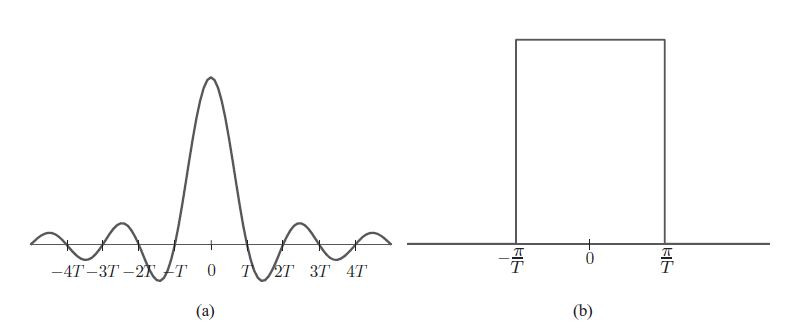
\includegraphics[scale = 0.5]{Figures/Sim_Fourier_Transform/sinc_rect_Fourier}
\caption{CTFT of $\text{sinc}\left(\,  \displaystyle\frac{t}{T}  \, \right)$ \cite{sampling_beyond_band_limited_systems}}
\label{fig:Sim_Fourier_Transform:sinc_rect_Fourier}
\end{figure}


\item Discrete Exponentials (section 3.3.2 in \cite{sampling_beyond_band_limited_systems}):

\begin{equation}
    x[n] \, = \, e^{j \, \omega_0 \, n} \leftrightarrow \, X(\omega) \, = \, 2 \pi \displaystyle\sum_{k \, \in \, \mathbb{Z}} \delta(\omega \, - \, \omega_0 \, + \, 2 \,  \pi \, k)
\end{equation}
    
\end{itemize}

\section{Continuous–discrete Representations}

\underline{Source:} See section 3.2 in \cite{sampling_beyond_band_limited_systems}.\\

In context of sampling, we deals with a \tbi{mixed signal representation}, involving 2 components: a continuous time signal $x(t)$ and a discrete time sequence $d[n]$, having the form:


\begin{equation}
    x(t) \, = \, \displaystyle\sum_{n \in \mathbb{Z}} d[n] \, h(t \, - \, n \, T_s)
\end{equation}

Some facts:

\begin{itemize}
    \item $X(\Omega) \, = \, D(\omega) \, H(\Omega)$
\end{itemize}



%********************************************
%********************************************
%********************************************



\chapter{$Z$ Transform}


\section{Some Preliminary:The $z$ number}


\begin{itemize}

\item complex number $z \, = \, r \, e^{j \, \Omega}$

\item If we form a signal called $x[k] \, = \, z^{k}$, it will be a \tbi{discrete time complex signal}, where using Euler identity we have:

\begin{equation*}
x[k] \, = \, z^{k} \, = \, r^k \, \left[\, \text{cos}(\Omega \, k) \, + \, \text{sin}(\Omega \, k)  \,\right]
\end{equation*}

	\begin{itemize}
	\item $r$ controls the damping of this signal
	
	\item and $\Omega$ controls the frequency

	\end{itemize}


\item For a complex exponential signal $z^k \, = \, (r \, e^{j \, \Omega})^k$ applied as input, we get the following response

\begin{equation}
\begin{array}{rcl}
y[k] \, &=& \, z^k \, \times \, \displaystyle\sum_{m \, = \, - \infty}^{+ \infty} h[m] \, \times \, z^m \\ \\
&=& \, H(z) \, \times \, z^k  
\end{array}
\end{equation}

	\begin{itemize}
	\item $z^k$ \tbi{eigenfunction} of the system with associated eigenvalue $H(z)$ 
	
	
	\item The signal  $z^k \, = \, (r \, e^{j \, \Omega})^k$ is called \tbi{eigenfunction} because an eigenfunction applied to a system, \tbi{give output = to the input but with a scaling factor}	
	
	\item In other words, and unlike normal sequences which can be decomposed into a combination of scaled and shifted impulses as $x[k] \, = \, \displaystyle\sum\limits_{n \, = \, - \infty}^{\infty} x[n] \, \delta[n \, - \, k]$, these sequences when getting passed through an LTI system will be changes, but exponential complex sequences $z^k$ \tbi{retain their shape}.	
	
	
	\end{itemize}

\newpage
\item As any complex number, $H(z) \, = \, |H(z)| \, e^{j \, \phi(z)}$, so we can further develop the response $y[k]$ as:

\begin{equation}
\begin{array}{rcl}
y[k] \, &=& \, z^k \, \times \, \displaystyle\sum_{m \, = \, - \infty}^{+ \infty} h[m] \, \times \, z^{-m} \\ \\
&=& \, H(z) \, \times \, z^k \\ \\
&=& |H(z)| \, e^{j \, \phi(z)}   \times \, z^k 
\end{array}
\end{equation}

	\begin{itemize}
	\item Interpretation: the system $H(z)$ \tbi{change only} the \tbi{amplitude} and the \tbi{phase} of the \tbi{input signal} $z^k$
	
	\item But it \tbi{won't change its frequency} $\Omega$
	\end{itemize}

\item As a special case, we can apply the same case for DTFT case: if we have a complex exponential signal at a certain discrete frequency $\omega_0$, we obtain the same signal, but modulated with transfer function $H(\omega_d)$:

\begin{equation}
y[k] \, = \, H(\omega_d) \, \times \, e^{j \, \omega_0 \, k}        
\end{equation}

\end{itemize}

\section{$Z$-Transform Definitions}


\begin{itemize}

\item  The \tbi{bilateral $z$-transform} of a discrete time signal $x[k]$ is:

\begin{equation}
X(z) \, = \, \displaystyle\sum_{k \, = \, - \infty}^{+ \infty} x[k] \, \times \, z^{-k}
\label{Eq:z_transform:definition_bilateral} 
\end{equation}


\item  The \tbi{inverse bilateral z-transform} of a $X[z]$ is:

\begin{equation}
x[k] \, = \, \displaystyle\frac{1}{2 \, \pi \, j} \displaystyle\oint X(z) \, z^{k \, - \, 1} \, dz
\end{equation}


\end{itemize}



\section{Convergence}

\begin{itemize}


\item The $z$-transform definition involves \tbi{infinite summation}

	\begin{itemize}
	\item Whenever we do an infinite sum, we ask the question  \tbi{when does this sum converge} ?
	\end{itemize}
	
	
\item Recall that $z \, = \, r \, e^{j \, \Omega}$

	\begin{itemize}
	\item Back to the definition of $z$-transform, the sum will converge if we have if the product $x[k] \, \times \, z^{-k}$ is \tbi{absolute summable}

	\item $\displaystyle\sum_{k \, = \, - \infty}^{+ \infty} \lvert \,x[k] \,r^{-k} \,\rvert \, < \, \infty \leftrightarrow$  Values of $r$ for which we have convergence is called \tbi{region of convergence}
	
	\begin{itemize}
	    \item The convergence is controlled by the magnitude of $z$ equal to $r$
	\end{itemize}
	

\end{itemize}		 


\end{itemize}


\newpage
\section{Region of Convergence}


\begin{itemize}

\item Definition of ROC: the set of $z$ values for which \autoref{Eq:z_transform:definition_bilateral} converges

\item Always Recall the rule: when using $X(z)$, we must \tbi{specify the region of convergence} for \tbi{unique correspondence} to a discrete time signal $x[k]$ 

	\begin{itemize}
	\item ROC \tbi{can't contains any pole} since it makes the $z$-transform tends to $\infty \, \leftrightarrow \, $ so no convergences
	\end{itemize}

\item Summary of Examples and their different region of convergence

\begin{figure}[h]
\centering
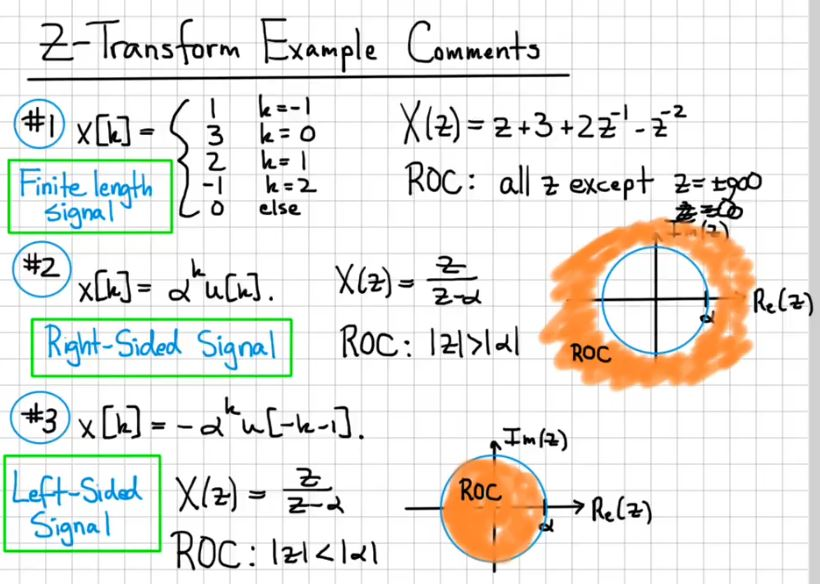
\includegraphics[scale=0.3]{Figures/z_transform/summary_examples}
\label{fig:z_transform:summary_examples}
\end{figure}


\item Different Type of discrete time signal and their correspondent ROC

	\begin{enumerate}
	\item Finite duration  $\leftrightarrow$ all the $z$-plane except for 0 and $\pm \infty$
	
		\begin{itemize}
		\item Example: a polynomial of $z$
		
		\item Intuition: when  working up with finite length signals, I will surely have convergence and stability.
		
		Problems comes from signals that keep up extending, like in next examples
		
		\end{itemize}
	
	\item Right sided signal $\leftrightarrow$ outside the circle
	
		\begin{itemize}
		\item Example: $x[k] \, = \, \alpha^k \, u[k] \, \leftrightarrow \, \displaystyle\frac{z}{z \, - \, \alpha}\quad $ ROC: $\lvert \, z \, \rvert \, > \, \alpha \leftrightarrow \text{Radius $>$ pole}$
		\end{itemize}
	
	\item Left sided signal $\leftrightarrow$ inside the circle
	
		\begin{itemize}
		\item  Example: $x[k] \, = \, - \, \alpha^k \, u[-k \, - \, 1] \, \leftrightarrow \, \displaystyle\frac{z}{z \, - \, \alpha}\quad $ ROC: $\lvert \, z \, \rvert \, < \, \alpha \leftrightarrow \text{Radius $<$ pole}$
		\end{itemize}
	
	\item Double sided signal $\leftrightarrow$ inside a ring (donate shape)
	\end{enumerate}


\item The double sided signal is the general case for an ROC, where $z$-transform exist for  $r_1 \, < \, \lvert z \rvert \, < \, r_2$, and the left sided and right sided are special case of the double sided (ring shape):
    
    \begin{itemize}
        \item Right sided $ \leftrightarrow \, \lvert z \rvert \, > \, r_1$
        
        \item Left sided $ \leftrightarrow \, \lvert z \rvert \, < \, r_2$
    \end{itemize}


\item Specify ROC: look how signals in example 2 and 3 have the same $z$-transform, but they have different ROC $\leftrightarrow$ always specify ROC when working with $z$-transform 

\end{itemize}


\section{$Z$-Transform Properties and Effect on ROC}

\begin{itemize}

\item when using $z-$transform \tbi{properties}, keep \tbi{track} at what happen to the \tbi{ROC for the final expression}

\item Review examples from slides

\item Pole-Zero cancellation and algebraic expression manipulation: we may end up with a bigger ROC of the final expression


\end{itemize}

\section{Inverse-$Z$ Transform}

\subsection{Partial Fraction Expansion}

\begin{itemize}

\item Ration of polynomials in function of $z^{- \, 1}$:

	\begin{equation}
	X(z) \, = \, \displaystyle\frac{B(z)}{A(z)}   \, = \, \displaystyle\frac{b_0 \, + \, b_1 \, z^{-1} \, + \, \cdots \, + \, b_M \, z^{- \, M}}{a_0 \, + \, a_1 \, z^{-1} \, + \, \cdots \, + \, a_N \, z^{- \, N}}
	\end{equation}
	
\item Express the ration $\displaystyle\frac{B(z)}{A(z)}$ as \tbi{linear combination of $1^{\mathrm{st}}$ order terms}:

	\begin{equation}
	X(z) \, = \, \displaystyle\sum\limits_{i \, = \, 1}^N\frac{A_i}{1 \, - \, d_i \, z^{-1}}
	\label{Eq:z_transform:first_order_terms}
	\end{equation}
	
	\begin{itemize}
	\item The nice thing about  \autoref{Eq:z_transform:first_order_terms} is we know their time domain expression
	\end{itemize}	

\item Concerning the $1^{\mathrm{st}}$ order $\frac{A_i}{1 \, - \, d_i \, z^{-1}}$ term, we have 2 choice as inverse $z$-transform:

	\begin{enumerate}
	\item $ \displaystyle\frac{A_i}{1 \, - \, d_i \, z^{-1}} A_i \, \leftrightarrow \, (d_i)^k \, \underbrace{u[k] }_{\text{right sided signal}} $ for an ROC $\underbrace{|z| \, > \, d_i}_{\text{Radius $>$ pole}}$
	
	\item  $ \displaystyle\frac{A_i}{1 \, - \, d_i \, z^{-1}} \, \leftrightarrow \, A_i \, (d_i)^k \, \underbrace{ u[\, -k \, - \, 1 \,] }_{\text{left sided signal}}\, $ for an ROC $|z| \, < \, d_i$
	\end{enumerate}


\item To \tbi{choose} the \tbi{correct discrete time domain expression}, we always need to \tbi{include} the \tbi{initial ROC of $X(z)$ before expansion}

	\begin{itemize}
	\item See Example in the slides
	\end{itemize}
	
\end{itemize}

\subsection{Long Division Method}

Another way we can do  inverse $z$-transform is \tbi{long division method}, which can be done when we have \tbi{1-sided signal}

	\begin{enumerate}
	\item if ROC \tbi{inside the unite circle} $\leftrightarrow \, |z| \, < \, a \leftrightarrow \, \text{right sided signal} \, \rightarrow$ we get a \tbi{sequence of positive power} of $z$ 
	
		\item if ROC \tbi{outside the unite circle} $\leftrightarrow \, |z| \, > \, a \, \leftrightarrow \, \text{left sided signal} \, \rightarrow$ we get a \tbi{sequence of negative power} of $z^{-1}$ 
	\end{enumerate}


\section{Causality and Stability}

\begin{itemize}

\item Location of the \tbi{pole} if it is \tbi{outside the unite circle}, we get either:

	\begin{enumerate}
	\item A decaying exponential $\leftrightarrow$ Non-causal but stable
	
	\item An increasing right sided exponential $\leftrightarrow$ Causal but not stable	
	\end{enumerate}

\item To ensure \tbi{stability and causality}:  \tbi{poles} must be \tbi{inside the unit circle}

\end{itemize}

\section{$Z$-Transform and Frequency Domain}

If we have some system with impulse response $h[k] \mapsto H(z)$, we can infer $H(\omega_d)$ from pole-zero plot, if the ROC include the unit circle, because we will evaluate $H(\omega_d)$ for different values of $z$ on the unit circle.\\

This is used in filter design.\\

Another thing: location of poles and zeros give us constraints about the requirement to design  the filter.



\section{Inverse Linear System and Minimum Phase}

\begin{itemize}

\item When designing real word system, we want them to be \textcolor{red}{causal} and \textcolor{red}{stable}

\item Dealing with \textcolor{red}{$H_{\text{inv}}(z)$}, they have the \textcolor{red}{flipped poles and zeros of $H(z)$}

\item So if we want $H_{\text{inv}}(z)$ to be causal and stable, the \textcolor{red}{poles} and \textcolor{red}{zeros} of $H(z)$ must be \textcolor{red}{inside the unit circle}


\item Definition:

A system $H(z)$ having \tbi{all its poles and zeros inside the unit circle} is called a \tbi{minimum phase system}

\end{itemize}


\section{Intuitions and Observations}

\subsection{Advantages of using $Z$-Transform}

\begin{enumerate}
    \item Applied to a more general class of signals, similar to Laplace transform
    
    \item We obtain allot of polynomials or rational function in $z$, which are more easier to track then complex exponential as in DTFT
    
    
    \item Essential when designing filter: designing directly filter in frequency domain can be difficult, but doing so in the $z$ domain is easier (to be seen later).
\end{enumerate}


\subsection{Why $z$-transform tables are in negative power}


\begin{itemize}
\item  If we look to the unilateral definition of $z$-transform, we obtain $X(z) \, = \,  \displaystyle\sum_{k \, = \, 0}^{+ \, \infty} x[k] \, z^{-k} \, = \, x[0] \, + \, x[1] \, z^{-1} \, + \, x[2] \, z^{-2} \, + \, \cdots$.

So for causal signals, all the $z$ numbers are in negative power, that's why by convention tables in references use negative power notation.\\
    
    
\item However, the downside of this is that we can't easily infer the poles and zeros of $X(z)$, we need to convert them to positive power of $z$.

\end{itemize}


\subsection{About Inverse $Z$-Transform}

\todo{To be seen later}.\\

In case we have a rational function $X(z)$, and want to use the tables to find the discrete time signal $x[k]$, we want that the degree in the denominator is bigger then the degree in the numerator.\\

If not, we extract the extra power in the numerator and make them as delays.\\

Video: 33:32.


%********************************************
%********************************************
%********************************************

\chapter{Introduction to Discrete Time Filters}



\section{Filter Desing Problems}

5 stages for filter design problems \cite{DSP_DimitrisManolakis}:

\begin{enumerate}
    \item Specification: frequency response characteristics for the application
    
    \item Approximation: approximate the desired frequency response (usually the ideal) by a practical frequency response of a filter having either a polynomial (FIR) or a rational system function (IIR)
    
    
    \item Quantization
    
    \item Verification: if not, repeat step 2 or reduce the filter performance requirement
    
    \item Implementation: implementing the system using software, hardware or both (in \autoref{Chap:DT_Impementation})
    
\end{enumerate}


\newpage
\section{Specification}


\begin{figure}[h]
\centering
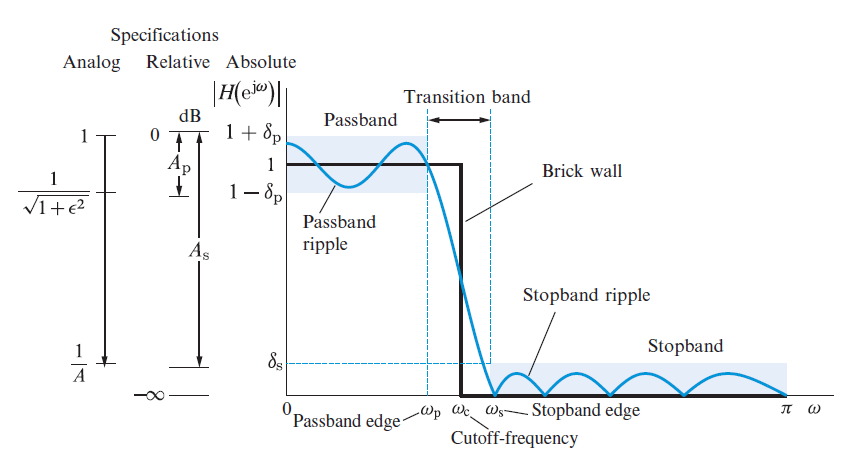
\includegraphics[scale=0.95]{Figures/FIR/spec_filter}
\label{fig:FIR:spec_filter}
\caption{Tolerance diagram for filter design specification \cite{DSP_DimitrisManolakis}}
\end{figure}


\section{Linear Phase Concept}

\begin{itemize}

\item An FIR has a linear phase if its impulse response has symmetry

\begin{equation}
    h[n] \, = \, \pm \, h[M \, - \, 1 \, - \, n] \quad \text{for } n \, = \, 0 \, , \, 1 \, , \, \cdots \, , \, M \, - \, 1
\label{Eq:FIR:FIR_Symmetry_Impulse_Response}
\end{equation}

The $+$ is symmetric and $-$ is antisymmetric

\end{itemize}

%********************************************
%********************************************
%********************************************

\chapter{FIR}


\section{Generalities}

\subsection{Recap of Equations}

\begin{itemize}

\item FIR Difference Equation: Output at some index $n$



\begin{equation}
\begin{array}{rcl}
  
  y[ \, n \,] \, &=& \, \displaystyle\sum\limits_{i \, = \, 0}^{M \, - \, 1} h[\,i \,] \, x[\, i \, - \, n\, ] \\ \\
     &=& \, b_0 \, x[n] \, + \, b_1 \, x[n \, - \, 1] \, + \, \cdots \, b_{M \, - \, 1} \, x[n \, - \, M \, +1]
\end{array}    
\end{equation}


\item FIR impulse response $h[n]$

\begin{equation}
\begin{array}{rcl}
   h[n] \, &=&  \, \begin{cases}
    b_n \quad n \, = \, 0 \, , \, 1 \, , \, \cdots \, , \, M \, - \, 1 \\ \\
    0 \quad \text{otherwise}
    \end{cases} \\ \\
    H(z) \, &=& \, \displaystyle\sum\limits_{i \, = \, 0}^{M \, - \, 1} h[\,n \,] \, z^{-n} \\ \\
     &=& \, \displaystyle\sum\limits_{i \, = \, 0}^{M \, - \, 1} b_n \, z^{-n} \\ \\
     H(\omega_d) \, &=& \, \displaystyle\sum\limits_{i \, = \, 0}^{M \, - \, 1} h[\,n \,] \, e^{-j \omega_d k} \\ \\
    &=& \, \displaystyle\sum\limits_{i \, = \, 0}^{M \, - \, 1} b_n \, e^{-j \omega_d k}
\end{array}
\end{equation}


\end{itemize}

\newpage
\subsection{Design Methods}

\begin{itemize}
    \item Time domain technique: window method
    
    
    \item Frequency domain methods: frequency sampling and Equiripple method
\end{itemize}


\section{Window Design Technique}

\underline{Key Ideas:}\\

\begin{itemize}

\item Truncation the non-causal part of the filter (before 0), and truncation the symmetrical part after 0 to preserve symmetry

    \begin{itemize}
        \item Truncation comes from the fact that the mean square error (optimization criterion used to find the FIR coefficients) is optimum if we truncate
    \end{itemize}


\item Filter taps $b_n$:

\begin{equation}
    b_n \, = \, \displaystyle\frac{B}{\pi} \, \times \, \text{sinc}\left[\, \frac{B}{\pi} \, \times \, \frac{n \, - \, N}{2}    \,\right]
\end{equation}

\item Difference Equation

\begin{equation}
    y[n] \, = \, b_0 \, x[n] \, + \, b_1 \, x[n \, - \, 1] \, + \, \cdots \, b_{N} \, x[n \, - \, N \, ]
\end{equation}

\item Impulse response $H(z)$

\begin{equation}
    H(z) \, = \, b_0 \, + \, b_1 \, z^{-1} \, + \, \cdots \, + \, b_N z^{-N}
\end{equation}


\item Window Effect of the response of the filter:

    \begin{itemize}
        \item Mainlobe $\rightarrow$ transition bandwidth
        
        \item Sidelobes $\rightarrow$ passband + stopband ripples
    \end{itemize}



\item Advantage: when increasing $N$, sharper transition band

\item Disadvantage: ripples won't be enhanced even if $N$ increase


    \begin{itemize}
        \item To use other methods different then rectangular to reduce sidelobes effect at the expense of a wider main lobe (wider transition bandwidth)
    \end{itemize}

\item Other disadvangatges of the window method:

    \begin{enumerate}
        \item Equal size ripples in each band $\rightarrow$ we cannot weight the passband and stopband ripples differently, even if most application require smaller ripples in the stopband
        
        \item Because of the frequency convolution, we cannot specify the edges and maximum ripple size of each band precisely
        
        \item Windowing method is sub-optimal because the designed filters do not satisfy the mean square error optimization criteria
        
    \end{enumerate}



\end{itemize}


\todo{To do tmrw}:\\

\begin{itemize}
    \item Write the hilighted information
    
    
    \item Understand how to compute the parameter of the windowing operation by frequency convolution
\end{itemize}

\section{Frequency Sampling Method}

Why using this method?

\begin{itemize}
    \item Window method required analytical expression to find the designed filter
    
       \begin{itemize}
           \item Recall that FIR using windowing required to find the frequency convolution operation between the ideal approximated filter and the DTFT of the window
           
           \begin{equation}
               H_{\text{FIR}}(\omega) \, = \, \displaystyle\frac{1}{2 \pi} \displaystyle\int\limits_{-\pi}^{\pi} H_{\text{ideal}}(\omega) \,  W(\omega \, - \, \theta) \,  d\omega
               \label{Eq:FIR:window_method_freq_convolution}
           \end{equation}
           
           
    \item Sometimes the analytical expression of $W(\omega)$ ($w[n]$) are not available, and all we have are some frequency samples to design our filter
           
       \end{itemize}
    

\item In windowing method, FIR filter is made by truncating the ideal filter $h_{\text{ideal}}[n]$, whereas in frequency sampling method FIR is made by aliasing of folding $h_{\text{ideal}}[n]$

\item In comparison to \autoref{Eq:FIR:window_method_freq_convolution}, frequency response $H_{\text{FIR}}(\omega)$ is obtained by interpolating between the samples of $H_{\text{ideal}}(\omega)$ and $W(\omega)$ as interpolating function via \autoref{Eq:FIR:freq_sampling_method}.

\begin{equation}
               H_{\text{FIR}}(\omega) \, = \, \displaystyle\frac{1}{L} \displaystyle\sum\limits_{k \, = \, 0}^{L \, - \, 1} H_{\text{ideal}}(k) \,  W \left(\omega \, - \, \displaystyle\frac{2 \pi k}{L} \right)
                \quad k \, = \, 0 \, , \, 1 \, \cdots \, , \, L \, - \, 1
                \label{Eq:FIR:freq_sampling_method}
           \end{equation}
    
where $L$: number of the given frequency samples equally spaced on the unit circle     
    
\end{itemize}


%********************************************
%********************************************
%********************************************


\chapter{IIR}



%********************************************
%********************************************
%********************************************

\chapter{Discrete Time Syteme Realization}
\label{Chap:DT_Impementation}

%********************************************
%********************************************
%********************************************

\chapter{Multirate Signal Processing}


\section{Downsampling}

\begin{itemize}
    
\item Downsampling is when we throw samples in discrete time domain

    \begin{itemize}
        \item Whereas undersampling is the term used when we sample below Nyquiste Rate
    \end{itemize}

\item Doing downsampling doesn't mean necessarily that aliasing will occur
    
    \begin{itemize}
        \item Recall that aliasing here is in the \tbi{discrete frequency domain} $\leftrightarrow$ DTFT spectrum where frequency $\in \, [ \, -\pi \, , \, +\pi \, ]$
    \end{itemize}


\end{itemize}

\begin{table}[!h]
\centering
	\begin{tabular}{|c|c|}
	\hline
		% header
		\multicolumn{2}{|c|}{Dowsampling}\\ \hline
		CTFT & DTFT \\ \hline
		
		Closer Images & Closer Images  \\ \hline
		
		Scaling Factor decrease & Scaling Factor decrease \\ \hline
		Bandwidth Same & Bandwidth Stretch \textcolor{blue}{but} still in $[\, - \, \pi , + \, \pi \,]$ \\ \hline		
	\end{tabular}
	\caption{Downsampling Operation Effects}
\end{table}


%********************************************
%********************************************
%********************************************

\chapter{Compressed Sensing}

\begin{itemize}

\item We always store information in a compressed way, such that the human perception system (visual or by hearing) won't make the difference

\item In case we get higher in dimensionality (images and video), the rate of compression will get higher due to redundancy in higher dimensional signal 


\item Sparse signals may have the benefit to differentiate between useful components and noisy components just by threshold

	\begin{itemize}
	\item Even if the signal is not sparse, we can use some sparse transformation and reduce noise in the transformed domain then do the reconstruction
	\end{itemize}

\end{itemize}

\section{Matrices and Notations}

\begin{itemize}

\item Let $\Vec{x}_{n \, \times \, 1}$ be a sparse vector in some basis $\Psi_{n \, \times \, n}$

    \begin{itemize}
        \item In our case, $\Vec{x}_{n \, \times \, 1}$ is a FT of some $\Vec{y}_{n \, \times \, 1}$ in the time domain
        
        \item the basis will be inverse DFT $ \leftrightarrow \Psi_{n \, \times \, n} \, = \, \text{F}^{-1} $
        
        \item $K$ is the maximum number of non-zero elements in $\Vec{x}_{n \, \times \, 1} \leftrightarrow \, \lVert \Vec{x} \rVert_0 \,  = \, K$
        
        
    \end{itemize}

\item Acquisition via the CS scheme:

\begin{equation}
\begin{array}{lll}
     \Vec{y}_{m \, \times \, 1} \, &=& \, \text{A}_{m \, \times \, n} \, \Vec{x}_{n \, \times \, 1} \\ \\
      &=& \, \textbf{R}_{m \, \times \, n} \,  \boldmath\Phi_{n \, \times \, n} \, \boldsymbol\Psi_{n \, \times \, n} \, \Vec{x}_{n \, \times \, 1} 
\end{array}
\end{equation}

such that $m \, \ll \, n$


\end{itemize}





\bibliographystyle{IEEEtran}
\bibliography{Literature/Books_Signal_Processing}

\end{document}


